% ========================================
%	Header einbinden
% ========================================

\documentclass[bibtotoc,titlepage]{scrartcl}

% Deutsche Spracheinstellungen
\usepackage[ngerman,german]{babel, varioref}
\usepackage[T1]{fontenc}
\usepackage[utf8]{inputenc}

%\usepackage{marvosym}

\usepackage{amsfonts}
\usepackage{amssymb}
\usepackage{amsmath}
\usepackage{amscd}
\usepackage{amstext}
\usepackage{float}
\usepackage{caption}
\usepackage{wrapfig}
\usepackage{setspace}
\usepackage{threeparttable}
\usepackage{footnote}

\usepackage{caption}
\usepackage{subcaption}

\newfloat{formel}{htbp}{for}
\floatname{formel}{Formel}


\usepackage{longtable}

%\usepackage{bibgerm}

\usepackage{footnpag}

\usepackage{ifthen}                 %%% package for conditionals in TeX
\usepackage{siunitx}
%Fr textumflossene Bilder und Tablellen
%\usepackage{floatflt} - veraltet

%Fr Testzwecke aktivieren, zeigt labels und refs im Text an.
%\usepackage{showkeys}

% Abstand zwischen zwei Abs�zen nach DIN (1,5 Zeilen)
% \setlength{\parskip}{1.5ex plus0.5ex minus0.5ex}

% Einrckung am Anfang eines neuen Absatzes nach DIN (keine)
%\setlength{\parindent}{0pt}

% R�der definieren
% \setlength{\oddsidemargin}{0.3cm}
% \setlength{\textwidth}{15.6cm}

% bessere Bildunterschriften
%\usepackage[center]{caption2}


% Probleml�ungen beim Umgang mit Gleitumgebungen
\usepackage{float}

% Nummeriert bis zur Strukturstufe 3 (also <section>, <subsection> und <subsubsection>)
%\setcounter{secnumdepth}{3}

% Fhrt das Inhaltsverzeichnis bis zur Strukturstufe 3
%\setcounter{tocdepth}{3}

\usepackage{exscale}

\newenvironment{dsm} {\begin{displaymath}} {\end{displaymath}}
\newenvironment{vars} {\begin{center}\scriptsize} {\normalsize \end{center}}


\newcommand {\en} {\varepsilon_0}               % Epsilon-Null aus der Elektrodynamik
\newcommand {\lap} {\; \mathbf{\Delta}}         % Laplace-Operator
\newcommand {\R} { \mathbb{R} }                 % Menge der reellen Zahlen
\newcommand {\e} { \ \mathbf{e} }               % Eulersche Zahl
\renewcommand {\i} { \mathbf{i} }               % komplexe Zahl i
\newcommand {\N} { \mathbb{N} }                 % Menge der nat. Zahlen
\newcommand {\C} { \mathbb{C} }                 % Menge der kompl. Zahlen
\newcommand {\Z} { \mathbb{Z} }                 % Menge der kompl. Zahlen
\newcommand {\limi}[1]{\lim_{#1 \rightarrow \infty}} % Limes unendlich
\newcommand {\sumi}[1]{\sum_{#1=0}^\infty}
\newcommand {\rot} {\; \mathrm{rot} \,}         % Rotation
\newcommand {\grad} {\; \mathrm{grad} \,}       % Gradient
\newcommand {\dive} {\; \mathrm{div} \,}        % Divergenz
\newcommand {\dx} {\; \mathrm{d} }              % Differential d
\newcommand {\cotanh} {\; \mathrm{cotanh} \,}   %Cotangenshyperbolicus
\newcommand {\asinh} {\; \mathrm{areasinh} \,}  %Area-Sinus-Hyp.
\newcommand {\acosh} {\; \mathrm{areacosh} \,}  %Area-Cosinus-H.
\newcommand {\atanh} {\; \mathrm{areatanh} \,}  %Area Tangens-H.
\newcommand {\acoth} {\; \mathrm{areacoth} \,}  % Area-cotangens
\newcommand {\Sp} {\; \mathrm{Sp} \,}
\newcommand {\mbe} {\stackrel{\text{!}}{=}}     %Must Be Equal
\newcommand{\qed} { \hfill $\square$\\}
\renewcommand{\i} {\imath}
\def\captionsngerman{\def\figurename{\textbf{Abb.}}}

%%%%%%%%%%%%%%%%%%%%%%%%%%%%%%%%%%%%%%%%%%%%%%%%%%%%%%%%%%%%%%%%%%%%%%%%%%%%
% SWITCH FOR PDFLATEX or LATEX
%%%%%%%%%%%%%%%%%%%%%%%%%%%%%%%%%%%%%%%%%%%%%%%%%%%%%%%%%%%%%%%%%%%%%%%%%%%%
%%%
\ifx\pdfoutput\undefined %%%%%%%%%%%%%%%%%%%%%%%%%%%%%%%%%%%%%%%%% LATEX %%%
%%%
\usepackage[dvips]{graphicx}       %%% graphics for dvips
\DeclareGraphicsExtensions{.eps,.ps}   %%% standard extension for included graphics
\usepackage[ps2pdf]{thumbpdf}      %%% thumbnails for ps2pdf
\usepackage[ps2pdf,                %%% hyper-references for ps2pdf
bookmarks=true,%                   %%% generate bookmarks ...
bookmarksnumbered=true,%           %%% ... with numbers
hypertexnames=false,%              %%% needed for correct links to figures !!!
breaklinks=true,%                  %%% breaks lines, but links are very small
linkbordercolor={0 0 1},%          %%% blue frames around links
pdfborder={0 0 112.0}]{hyperref}%  %%% border-width of frames
%                                      will be multiplied with 0.009 by ps2pdf
%
%\hypersetup{ pdfauthor   = {Hannes Franke; Julius Tilly},
%pdftitle    = {x}, pdfsubject  = {Protokoll FP}, pdfkeywords = {V301, Innenwiderstand, Leistungsanpassung},
%pdfcreator  = {LaTeX with hyperref package}, pdfproducer = {dvips
%+ ps2pdf} }
%%%
\else %%%%%%%%%%%%%%%%%%%%%%%%%%%%%%%%%%%%%%%%%%%%%%%%%%%%%%%%%% PDFLATEX %%%
%%%
\usepackage[pdftex]{graphicx}      %%% graphics for pdfLaTeX
\DeclareGraphicsExtensions{.pdf}   %%% standard extension for included graphics
\usepackage[pdftex]{thumbpdf}      %%% thumbnails for pdflatex
\usepackage[pdftex,                %%% hyper-references for pdflatex
bookmarks=true,%                   %%% generate bookmarks ...
bookmarksnumbered=true,%           %%% ... with numbers
hypertexnames=false,%              %%% needed for correct links to figures !!!
breaklinks=true,%                  %%% break links if exceeding a single line
linkbordercolor={0 0 1},
linktocpage]{hyperref} %%% blue frames around links
%                                  %%% pdfborder={0 0 1} is the default
% \hypersetup{
% pdftitle    = {V301 Innenwiderstand und Leistungsanpassung}, 
% pdfsubject  = {Protokoll AP}, 
% pdfkeywords = {V301, Innenwiderstand, Leistungsanpassung},
% pdfsubject  = {Protokoll AP},
% pdfkeywords = {V301, Innenwiderstand, Leistungsanpassung}}
%                                  %%% pdfcreator, pdfproducer,
%                                      and CreationDate are automatically set
%                                      by pdflatex !!!
\pdfadjustspacing=1                %%% force LaTeX-like character spacing
\usepackage{epstopdf}
%
\fi %%%%%%%%%%%%%%%%%%%%%%%%%%%%%%%%%%%%%%%%%%%%%%%%%%% END OF CONDITION %%%
%%%%%%%%%%%%%%%%%%%%%%%%%%%%%%%%%%%%%%%%%%%%%%%%%%%%%%%%%%%%%%%%%%%%%%%%%%%%
% seitliche Tabellen und Abbildungen
%\usepackage{rotating}
\usepackage{ae}
\usepackage{
  array,
  booktabs,
  dcolumn
}
\makeatletter 
  \renewenvironment{figure}[1][] {% 
    \ifthenelse{\equal{#1}{}}{% 
      \@float{figure} 
    }{% 
      \@float{figure}[#1]% 
    }% 
    \centering 
  }{% 
    \end@float 
  } 
  \makeatother 


  \makeatletter 
  \renewenvironment{table}[1][] {% 
    \ifthenelse{\equal{#1}{}}{% 
      \@float{table} 
    }{% 
      \@float{table}[#1]% 
    }% 
    \centering 
  }{% 
    \end@float 
  } 
  \makeatother 
%\usepackage{listings}
%\lstloadlanguages{[Visual]Basic}
%\allowdisplaybreaks[1]
%\usepackage{hycap}
%\usepackage{fancyunits}
\usepackage{xfrac}
\usepackage{xcolor}
\usepackage{setspace}\usepackage{threeparttable}
\usepackage{fancyhdr}
\usepackage{graphicx}
\usepackage[official]{eurosym}
\usepackage{geometry}
\newcommand{\ti}{\text{i}}
\usepackage{siunitx}
\sisetup{output-decimal-marker = {,}}

% ========================================
%	Angaben für das Titelblatt
% ========================================

\title{V49 - Messung von Diffusionskonstanten mittels gepulster Kernspinresonanz\\
\hspace{15cm}% Titel des Versuchs 
	\large TU Dortmund, Fakultät Physik\\ 
	\normalsize Fortgeschrittenen-Praktikum}

\author{Dimitrios Skodras\\			% Name Praktikumspartner A
	{\small \href{dimitrios.skodras@tu-dortmund.de}{dimitrios.skodras@tu-dortmund.de}}	% Erzeugt interaktiven einen Link
	\and						% um einen weiteren Author hinzuzfügen
	Julius Tilly\\					% Name Praktikumspartner B
	{\small \href{julius.tilly@tu-dortmund.de}{julius.tilly@tu-dortmund.de}}		% Erzeugt interaktiven einen Link
}
\date{12.12.2016}				% Das Datum der Versuchsdurchführung

% ========================================
%	Das Dokument beginnt
% ========================================

\begin{document}
	
% ========================================
%	Titelblatt erzeugen
% ========================================

\maketitle					% Jetzt wird die Titelseite erzeugt
\thispagestyle{empty} 				% Weder Kopfzeile noch Fußzeile

% ========================================
%	Der Vorspann
% ========================================

%\newpage					% Wenn Verzeichnisse auf einer neuen Seite beginnen sollen
%\pagestyle{empty}				% Weder Kopf- noch Fußzeile für Verzeichnisse

\tableofcontents

%\newpage					% eine neue Seite
%\thispagestyle{empty}				% Weder Kopf- noch Fußzeile für Verzeichnisse
%\listoffigures					% Abbildungsverzeichnis

%\newpage					% eine neue Seite
%\thispagestyle{empty}				% Weder Kopf- noch Fußzeile für Verzeichnisse
%\listoftables					% Tabellenverzeichnis
\newpage					% eine neue Seite


% ========================================
%	Kapitel
% ========================================

\section{Theoretische Grundlagen}
\setcounter{page}{1}
Kernspinresonanz beschreibt die Messung der makroskopischen Magnetisierung, erzeugt durch ein äußeres Magnetfeld, abhängig vom Kernspin der
untersuchten Probe.
\subsection{Kernspinresonanz}
Dieses Magnetfeld $\vec B=B_0\vec z$ verursacht die Aufspaltung der entarteten Kernspinzustände in $2I+1$ Unterniveaus mit je 
$\Delta E = \gamma B_0 \hbar$ zueinander. Hierbei sind $I$ die Kernspinquantenzahl und $\gamma$ das gyromagnetische Moment. Für Wasserstoff ist
$I=\sfrac12$, also gibt es zwei Unterniveaus mit den Orientierungsquantenzahlen $m=\pm\sfrac12$, die nach der Boltzmann-Verteilung ungleich besetzt 
sind $\sim\exp\left(-\Delta E/kT\right)$.
Dadurch entsteht eine Kernspinpolarisation $\langle I_z \rangle$, die mit $\Delta E \ll kT$ berechnet werden kann. 
Die einzelnen magnetischen Momente $\vec \mu_I$ der einzelnen Kerne werden nun zur makroskopischen Magnetisierung $\vec M_0$ der Probe aufsummiert,
mit ihrem Erwartungswert in $z$-Richtung $\langle M_0\rangle = N \gamma \mu_0 \langle I_z\rangle$. Hierbei ist $N$ die Anzahl der Momente pro Volumen.
Gemessen wird die Magnetisierung durch das Auslösen ihrer Ruhelage mittels eines Hochfrequenzpulses (HF). Diese präzediert um das äußere Magnetfeld,
ausgedrückt durch die Differenzialgleichung
\begin{align}
 \frac{\dx}{\dx t}\vec M = \gamma \vec M \times B_0 \vec z.
 \label{eq:Mdgl}
\end{align}
Ihre Komponenten $M_x$ und $M_y$ beschreiben eine Kreisbewegung mit der Frequenz $\omega_L := \gamma B_0$, der Larmor-Frequenz. Nachdem
der HF-Puls die Magnetisierung gestört hat, strebt sie wieder ihrem Ursprungszustand $\vec M_0$ entgegen, sie relaxiert. Die Relaxation
und die Präzession zusammengefasst ergeben die Bloch-Gleichungen
\begin{align}
 \frac{\dx}{\dx t}M_x &= \omega_L M_y - \frac{M_x}{T_2},\\
 \frac{\dx}{\dx t}M_y &= \omega_L M_x - \frac{M_y}{T_2},\\
 \frac{\dx}{\dx t}M_z &= \frac{M_0-M_z}{T_1},
 \label{eq:bloch}
\end{align}
mit den Relaxationszeiten $T_1$ und $T_2$. Diese beschreiben den Energieübergang aus dem Spinsystem ins Gitter, bzw. die Wechselwirkung
benachbarter Spins. \\
\noindent Die genannten HF-Pulse werden von einem Signalgenerator bei der Larmorfrequenz erzeugt und für eine bestimmte Pulslänge 
$\Delta t_\delta$ an eine Spule geleitet, die ein Magnetfeld $\vec B_\text{HF} = 2\vec B_1 \cos(\omega t)$ generiert. Dieses ist senkrecht
zu und präzediert um $\vec z$ und kann zusammen mit $B_0$ als $B_\text{ges}$ geschrieben werden. In einem mit $\omega$ um $\vec z$ 
rotierenden Koordinatensystem $\{\vec x', \vec y', \vec z\}$ ist das $B_1$-Feld zeitlich konstant, welches o.B.d.A in $\vec x'$ Richtung zeigt. 
Da nun $\vec x' = \vec x'(t)$, ergibt sich für 
\eqref{eq:Mdgl}
\begin{align}
 \frac{\dx }{\dx t}\vec M = \gamma \vec M  \times \left(\vec B_\text{ges} + \frac{\vec \omega}{\gamma}\right).
\end{align}
Hiermit lässt sich ein $\vec B_\text{eff} = \vec B_\text{ges} + \vec\omega/\gamma$ schreiben, um das sich $\vec M$ effektiv aus $\vec z$ herausdreht. Wenn
die eingestrahlte Frequenz gleich der Larmorfrequenz ist, ist $\vec \omega$ antiparallel zu $\vec z$ und folglich ist $\vec B_\text{eff}=\vec B_1$.
Die Dauer in der das Magnetfeld die Magnetisierung um den Winkel $\delta$ aus der $\vec z$-Achse dreht, ergibt sich nun zu
$\Delta t_\delta = \delta/\gamma B_1$.

\subsection{Messmethoden von den Relaxationszeiten und der Diffusionskonstanten}
Zur Bestimmung der Relaxationszeiten $T_1$ und $T_2$ wird die Magnetisierung, wie bereits beschrieben, in die $x'$-$y'$-Ebene mit einem 
$\sfrac{\pi}{2}$-Puls gebracht. Die Präzession der Magnetisierung induziert eine Spannung in der HF-Spule, die gemessen wird.
\subsubsection{Spin-Gitter-Relaxation}
Beginnend mit einem $\pi$-Puls wird die Gleichgewichtsmagnetisierung $M_0$ in $-\vec z$-Richtung gebracht. Diese geht nun wieder mit der Zeit 
in $+\vec z$-Richtung. Nach einer gewissen Wartezeit $\tau$ wird ein $\sfrac{\pi}{2}$-Puls erzeugt, womit eine Spannung proportional
zu
\begin{align}
 M_z(\tau) = M_0\left(1-2\exp\left(\frac{\tau}{T_1}\right)\right)
 \label{eq:T1}
\end{align}
induziert wird. Mit Messungen für diverse $\tau$ lässt sich $T_1$, die Spin-Gitter-Relaxationszeit, bestimmen.

\subsubsection{Spin-Spin-Relaxation}
Ähnlich simpel ist die Beschreibung der Spin-Spin-Relaxationszeit $T_2$ mit dem freien Induktionszerfall. Hierzu wird ein $\sfrac{\pi}{2}$-Puls
durchgeführt, woraufhin die Magnetisierung wieder zur Ruhelage tendiert. Die Induktionsspannung im Laufe der Zeit liefert die Bestimmung von $T_2$.
Durch Magnetfeldinhomogenitäten und Wechselwirkungen mit benachbarten Dipolfeldern jedoch, gibt es eine Verteilung von Larmorfrequenzen, was 
schneller bzw. langsamer präzedierenden Momenten enspricht. Diese Dephasierung lässt sich ausdrücken durch $T_{\Delta B}$ und beeinflusst
die $T_2$-Messung maßgeblich, wenn $T_{\Delta B} < T_2$. Diese Konstante wird beschrieben durch $T_{\Delta B} = 1/\gamma d G$ mit dem 
Probendurchmesser $d$ und $G$, dem $B_0$-Gradienten.\\
\noindent Eine erste Verbesserung dazu ist die Spin-Echo-Methode. Hierzu wird der Dephasierung nach einer Zeit $\tau $ mit einem $\pi$-Puls 
entgegengewirkt, sodass die Momente wieder zusammenlaufen. Nach $2\tau$ wird eine Resonanz gemessen. Durch irreversible Dephasierungsprozesse
ist die gemessene Magnetisierung abhängig von $\tau$, ausgedrückt durch
\begin{align}
 M_y(\tau) = M_0\exp\left(-\frac{\tau}{T_2} \right).
 \label{eq:My}
\end{align}
Dieses Verfahren ist langwierig, da gewartet werden muss, bist die Magnetisierung wieder vollständig relaxiert ist. Die Carr-Purcell-Methode (CP)
fügt viele weitere $\pi$-Pulse bei $2n\tau$ ($n\in\mathbb{N}$) hinzu, wobei die Resonanzamplitude mit wachsendem $n$ abnimmt. Eine Fehlerquelle
hierin ist die Bedingung für exakt bestimmte $\Delta t_{\pi}$, denn anderweitig sind liegen die Momente um einen Winkel $\epsilon$ aus der 
$x'$-$y'$-Ebene heraus. Mit jedem $\pi$-Puls wird $\epsilon$ weiter addiert, sodass $T_2$ zu klein gemessen wird. Eine weitere Methode, die 
diesen Nachteil beseitigt, ist die Meiboom-Gill-Methode (MG). Ähnlich der CP-Methode werden die $\pi$-Pulse jedoch um $\pi/2$ gegen den 
$\pi/2$-Puls phasenverschoben, sodass $\vec B$ direkt zu Beginn in $\vec y'$-Richtung zeigt. Der überschüssige Winkel $\epsilon$ wird beim
zweiten $\pi$-Puls wieder negiert. Dieses Verfahren ist in Abbildung \ref{pic:MGmeth} dargestellt.
\begin{figure}[t]
 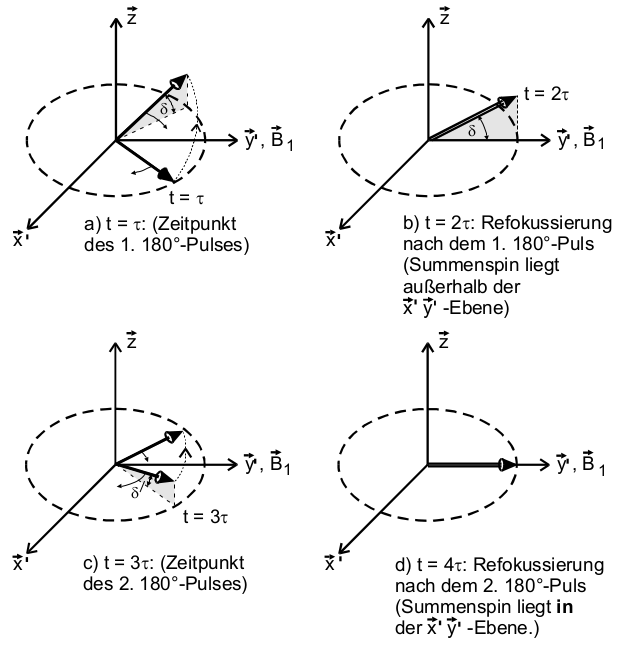
\includegraphics[width=.7\textwidth]{../pics/MG.png}
 \caption{Darstellung der Meiboom-Gill-Methode. Hier mit zwei Magnetisierungsvektoren zur Veranschaulichung der Dephasierung und $\epsilon=\delta$
 \cite{Anl}}
 \label{pic:MGmeth}
\end{figure}

\subsubsection{Einfluss der Diffusion}
Die $T_2$-Bestimmung mit \eqref{eq:My} gilt für lokal konstante $B_0$-Felder. In Flüssigkeiten ändern die spintragenden Teilchen ihren Ort
durch Brownsche Bewegung, was aufgrund von Feldinhomogenitäten zu zeitlich veränderlichen Larmorfrequenzen führt. Die Refokussierung wird
gestört und $M_y$ fällt schneller als durch \eqref{eq:My} beschrieben. Daher wird ein Diffusionsterm zu den Blochgleichungen \eqref{eq:bloch}
hinzugefügt. Die Diffusionsstromdichte $\vec j=-D\nabla n$ ist beschrieben durch die Änderung der Teilchendichte $n$ und der Diffusionskonstante $D$,
deren Bestimmung im weiteren ermittelt wird. Dieser Strom setzt sich für Protonen zusammen aus einem Strom parallel und einem antiparallelen zur
$\vec z$-Richtung. Die Magnetisierung $M=\mu(n_\text{p}-n_\text{a}$ und die Stromdichte der Momente 
$\vec J_M = \mu (\vec j_\text{p} - \vec j_\text{a}$ erfüllen eine Kontinuitätsgleichung, die für eine ortsunabhängige Diffusionskonstante 
\begin{align}
 \frac{\partial}{\partial t}M = -\nabla \vec J_M = D\Delta M
\end{align}
lautet, mit dem Laplaceoperator $\Delta = \nabla\cdot \nabla$. Zur Lösung der erweitereten Blochgleichungen des transversalen Anteils $M_\text{tr}$
wird ein Feld $B_z = B_0 + Gz$ mit dem örtlich konstanten Feldgradienten G angesetzt. Es folgt
\begin{align}
 \frac{\partial}{\partial t}M_\text{tr} = -\left(\frac{1}{T_2}+\ti\omega_L\right)M_\text{tr} - \left(\ti\gamma Gz - D\Delta\right)M_\text{tr},
 \label{eq:mtrDGL}
\end{align}
gelöst durch den Ansatz
\begin{align}
 M_\text{tr} = \exp\left(-\sfrac{t}{T_2}\right)\exp(\ti\omega_L t) f(x,y,z,t).
 \label{eq:mtransatz}
\end{align}
Die Funktion $f$ beschreibt den Gradienten- und den Diffusionsterm. Der Ansatz $f= A(t) \exp[-\ti\gamma Gz(t-2n\tau)]$ mit \eqref{eq:mtransatz}
liefert für die Zeitpunkte $t=2n\tau$ bei denen ein Echo erwartet wird
\begin{align}
 A(t) = \exp\left(-\frac13 D\gamma^2 G^2 \tau^2 t\right).
\end{align}
Eine neue Zeitkonstante $T_D = 3/D\gamma^2G^2 \tau^2\sim1/\tau^2$ beschreibt das Abfallen der Magnetisierung
\begin{align}
 M_y = M_0\exp\left(-\frac{t}{T_2}\right)\exp\left(-\frac{t}{T_D}\right).
 \label{eq:MyDiff}
\end{align}
Für kleine $\tau$ wird der Einfluss von $T_D$ klein und $T_2$ kann mit der CP- oder MG-Methode bestimmt werden. Jedoch kann hiermit auch 
die Diffusionskonstante errechnet werden unter der Betrachtung, dass die gemessene Spannung des Spin-Echos beschrieben wird durch
$U(\chi)\sim \sfrac{J_1(\chi)}{\chi}$ mit der Besselfunktion 1. Ordnung $J_1$ und $\chi:=\sfrac12 d G t$. Der Feldgradient berechnet sich nun aus 
der Beziehung $\sfrac14 d \gamma G t_{\sfrac12} = 2,2$ mit der zeitlichen Halbwertsbreite des Echos $t_{\sfrac12}$, woraufhin $D$ schließlich 
mithilfe von $T_2$ aus \eqref{eq:MyDiff} berechnet werden kann. Weiterhin kann der Molekülradius $r$ mit der Stokesgleichung
\begin{align}
 D = \frac{k_B T}{6\pi r \eta}
\end{align}
ermittelt werden. Die Viskosität $\eta$ wird experimentell bestimmt. Zwei Methoden zur theoretischen $r$-Berechnung werden zum Vergleich
vorgestellt. Unter der Betrachtung, dass die Moleküle hexagonal dicht gepackt (hcp) sind nehmen sie das Volumen 
$V_\text{hcp}=\sfrac{\pi}{3\sqrt{2}}\cdot\sfrac{m_T}{\rho}$ ein. Mit der molaren Masse $m_T=\SI{18.01528}{\g\per\mol}$, der Dichte 
$\rho = \SI{1,0}{\kg\per\m\cubed}$ \cite{conv} und der Kugelform ergibt sich
\begin{align}
 r_\text{hcp}=\left(\frac{3}{4\pi}\frac{V_\text{hcp}}{N_A} \right)^{\sfrac13} = \SI{1,74}{\angstrom}.
 \label{eq:radhcp}
\end{align}
Eine weiterer Weg führt über die van-der-Waals-Gleichung. Am kritischen Punkt, bei dem sich die Dichten der flüssigen und gasförmigen Phase 
angleichen, verschwinden die erste und zweite Ableitung des Drucks $p$ nach dem Volumen $V$ bei konstanter Temperatur $T$. Damit lassen sich
die kritischen Parameter $p_c$ und $T_c$ in Abhängigkeit der van-der-Waals-Parameter $a$ und $b$ ausdrücken. Für das kritische, molare 
Volumen gilt $V_c = b/4 = RT_c/32p_c$ mit der universellen Gaskontante $R=N_ak$. Für Wasser ist $T_c=\SI{647,1}{\K}$ und $p_c=\SI{22,12}{\MPa}$
\cite{chemie}. Der Radius ist nun
\begin{align}
 r_\text{vdW}=\left(\frac{3}{4\pi}\frac{V_\text{c}}{N_A}\right)^{\sfrac13} = \SI{1,44}{\angstrom}.
 \label{eq:radvdw}
\end{align}


\section{Durchführung}
Die Apparatur besteht aus einer Vorrichtung für den Permanentmagneten und die HF-Spule. Weiterhin gibt es einen PS2 Controller zur Einstellung
der Feldgradienten für $x$, $y$, $z$ und $z^2$. Mit dem Mainframe können die Frequenz des HF-Felds, die Pulslänge $A$, die Phase $\phi$, 
die Pulszwischenzeit $\tau$ und die Messmethode eingestellt werden. Ein Oszilloskop stellt die Echoamplitude dar.
\subsection{Justage}
Zu Beginn wird eine Wasserprobe eingeführt, die mit CuSO$_4$-Ionen versetzt ist, um $T_2$ zu verringern. Unter Manipulation der am Mainframe
einstellbaren Parametern soll ein FID ohne weitere Oszillationen erzeugt werden. Die Halbwertsbreite dafür soll zwischen \SI{1,5}{\ms} und
\SI{2,0}{\ms} liegen. Die erhaltenen Parameter lauten \footnote{Es zeigt sich, dass die Parameter mit der Zeit nachkalibriert werden müssen, da
das FID-Echo seine Form verändert.}
\begin{table}[h]
\begin{tabular}{l@{=}r}
 $\omega_L$ \quad& \quad\SI{21.67875}{\MHz},\\
 $\phi$ & +\SI{172}{\degree},\\
 $x$ & \SI{-1,52}{\tesla\per \m},\\
 $y$ & \SI{-6,17}{\tesla\per \m},\\
 $z$ & +\SI{2,63}{\tesla\per \m},\\
 $z^2$ & \SI{-0,60}{\tesla\per \m},\\
 $A$ & \SI{4,60}{\micro\second}.
\end{tabular}
\end{table}

\subsection{Spin-Gitter-Relaxationszeit}
\label{sec: T1}
Zur $T_1$-Messung wird ein Spin-Echo verwandt mit den Pulszeiten $\Delta t_{\pi} =: B = \SI{10,4}{\micro\second}$
und $\Delta t_{\sfrac{\pi}{2}} = A = \SI{4,6}{\micro\second}$, in dieser Reihenfolge.
Die Zeit zwischen zwei Messungen liegt bei \SI{10}{\second}. 
Im Bereich $\tau\in[0,05; 1,35]\SI{}{\second}$ wird 26 mal die Echoamplitude gemessen.
\subsection{Spin-Spin-Relaxationszeit}
\label{sec: T2}
Mit $N=100$ $\pi$-Pulsen nach dem $\sfrac{\pi}{2}$-Puls wird die CP-Methode mit $\tau = \SI{5.2}{\milli\second}$ durchgeführt und ein 
Bild des Amplitudenverlaufs gespeichert. Durch Umlegen des MG-Schalters am Mainframe wird die MG-Methode mit $\tau = \SI{13.5}{\milli\second}$ 
durchgeführt. Neben dem Amplitudenverlaufsbild werden die Datenpunkte zur weiteren Auswertung gespeichert.

\subsection{Diffusionskonstante}
\label{sec: diff}
Um die Diffusionskonstante zu bestimmen, muss $G$ bekannt sein. Hierzu wird ein künstlicher Feldgradient erzeugt, indem der $z$-Gradient maximal 
auf $-\SI{10}{\tesla\per\m}$ gestellt wird. Dieser lässt sich anschließend durch $t_{\sfrac12}$ näherungsweise angeben. Mit dem MG-Verfahren
werden nun die Amplituden für $\tau\in[1;23]\SI{}{\milli\second}$ ermittelt. Um den Molekülradius zu berechnen, wird die Viskosität gemessen
werden. Dies geschieht mithilfe eines Kapillarviskosimeters, in dem das Wasser von der ersten Kennlinie zur zweiten absinkt und die Zeit
dafür gemessen wird. Dieser wird ein Fehler $d(t)$ aus einer Tabelle zugeordnet und mit einem Koeffizienten $\alpha$ wird $\eta=\alpha\rho(t-d(t))$
berechnet.

\section{Auswertung}
\subsection{$T_1$-Zeit}

Die Messung der $T_1$-Zeit wird wie in Abschnitt \ref{sec: T1} beschrieben durchgeführt. Die Messwerte sind in Tabelle \ref{Tab:T_1} aufgeführt und nach Gleichung \ref{eq:T1} in der Abb. \ref{Abb:T_1} als $\ln \left( \frac{M_0-M_z}{2M_0}\right)$ gegen t dargestellt.


\begin{table}[htbp]
	\begin{center}
		\begin{tabular}{l|c||l|c}
			$\tau$[s] & Spannung[V] & $\tau$[s] & Spannung[V] \\ \hline
			\input{../auswertung/results/T1_tab.res}
		\end{tabular}
	\end{center}
	\caption{Auflistung der zur Bestimmung der $T_1$-Zeit in Abhänigkeit von $\tau$ aufgezeichneten Magnetisierungs Maxima.}
	\label{Tab:T_1}
\end{table}


\begin{figure}[H]
	\centering
	\vspace*{-0,85cm}
	\includegraphics[scale= 0.735]{../auswertung/results/T1.pdf}
	\caption{Darstellung der zur Bestimmung der $T_1$-Zeit in Abhänigkeit von $\tau$ aufgezeichneten Magnetisierungs Maxima. Die durch Ausgleichsrechnung erhaltene Gerade ist grün gestrichelt gekennzeichnet.}
	\label{Abb:T_1}
\end{figure}

\noindent
Es ergibt sich die $T_1$-Zeit aus der Steigung der Ausgleichsgeraden m$\cdot$x\\
mit $\input{../auswertung/results/m.res}$ nach $T_1 = -\frac{1}{m}$ zu:
\begin{center}
	$\input{../auswertung/results/T1.res}$
\end{center}
Der Fehler von $T_1$ wird über $\Delta T_1 = \frac{1}{m^2} \cdot \Delta m$ bestimmt.

\subsection{$T_2$-Zeit}

Um $T_2$ zu bestimmen wird wie in \ref{sec: T2} beschrieben vorgegangen. 
$T_2$ wird über die Meiboom-Gill-Methode bestimmt. Das zugehörige Zeitsignale ist in Abb. \ref{Abb:T_2_meiboom_gill} dargestellt.
Die Carr-Purcell-Methode ist für die $T_2$-Bestimmung dagegen nicht geeignet, da sich Fehleinstellungen der Pulse und somit der Flipwinkel mit jedem $ \SI{180}{\degree} $-Flip akkumulieren. Dies ist an den oszillierenden Amplituden in Abb. \ref{abb:carr_purcell} zu erkennen.

\begin{figure}[H]
	\includegraphics[width=\textwidth]{../auswertung/results/T2_carr_purcell.pdf}
	\caption{Vom Oszilloskop aufgenommene Messwerte des Carr-Purcell-Verfahrens. Aufgrund der sich addierenden Fehler enstehen Oszillationen des Spin-Echos.}
	\label{abb:carr_purcell}
\end{figure}

\begin{figure}[H]
	\centering
	\includegraphics[width=\textwidth]{../auswertung/results/T2.pdf}
	\caption{Vom Osziloskop aufgenommene Messwerte des Meiboom-Gill-Verfahrens mit Fit zur Bestimmung von $T_2$.}
	\label{Abb:T_2_meiboom_gill}
\end{figure}

Die in Abb. \ref{Abb:T_2_meiboom_gill} mit rotem Kreuz markierten Maxima werden für einen Fit mit
\begin{align*}
	U_{\text{fit}}(t) = U_0 \cdot \e^{-\frac{t}{T_2}},
\end{align*}
verwendet, welcher Mithilfe der Python Funktion \emph{scipy.optimize.curve\_fit()} ausgeführt wird.
Der Fit ergibt für $U_0$ und das gesuchte $T_2$
\begin{align*}
U_0 &= \input{../auswertung/results/T2_M0.res} \\
T_2 &= \input{../auswertung/results/T2.res}.
\end{align*}


\subsection{Diffusionskoeffizienten}
\label{Kap:Dif_koef}

Die Halbwertsbreite ergibt sich aus drei am Oszilloskop abgelesenen Breiten für verschiedene $\tau$ zu $t_{1/2}=\input{../auswertung/results/halfwidth.res}$.
Die verwandten Messdaten sind in Tab. \ref{Tab: Halfw} eingetragen.

\begin{table}[H]
	\begin{center}
		\begin{tabular}{l|c}
			$t_{1/2}$ & $\tau[\si{\milli\second}]$\\ \hline
			\input{../auswertung/results/halfw_tab.res}			
		\end{tabular}
	\end{center}
	\caption{Messwerte zur Bestimmung der Halbwertsbreite}
	\label{Tab: Halfw}
\end{table}

Zur Bestimmung des Diffusionskoeffizienten wird wie in Kapitel \ref{sec: diff} beschrieben die Magnetisierung in Abhänigkeit von $\tau$ bestimmt. Die hierfür aufgezeichneten Daten sind in der Tab. \ref{Tab:D} aufgelistet und werden zusammen mit der Ausgleichsgeraden in Abb. \ref{Abb:D} dargestellt.

\begin{table}[H]
	\begin{center}
		\begin{tabular}{l|c||l|c}
			$\tau$[ms] & Spannung[V] & $\tau$[ms] & Spannung[V]\\ \hline
			\input{../auswertung/results/diff_tab.res}
		\end{tabular}
	\end{center}
	\caption{Tabelle mit Messwerten zur Bestimmung des Diffusionskoeffizienten bei maximalem Z-Gradienten.}
	\label{Tab:D}
\end{table}

\begin{figure}[H]
	\centering
	\vspace*{-0,4cm}
	\includegraphics[scale= 0.74]{../auswertung/results/TDiff.pdf}
	\caption{Darstellung der zur Bestimmung des Diffusionskoeffizienten bei maximalem Z-Gradienten aufgezeichneten Magnetisierungs Maxima. Der lineare Fit ist grün-gestrichelt aufgetragen.}
	\label{Abb:D}
\end{figure}

\noindent
Ausgehend von Gleichung \ref{eq:MyDiff} folgt:
\begin{align*}
\ln \left( \frac{M_y (t)}{M_0} \right) + \frac{t}{T_2} = \frac{D\gamma^2 G^2}{12}t^3 ~\\
\overset{G= \frac{8.8}{t_{1/2}\gamma d}}{\Longrightarrow} \hspace*{0,5cm} \ln \left( \frac{M_y (t)}{M_0} \right) + \frac{t}{T_2} = \frac{484}{75}\frac{D t^3}{t^2_{1/2} d^2}
\end{align*}
Mit der Halbwertsbreite $\input{../auswertung/results/halfwidth.res}$ dem Probendurchmesser $d = 4.4\,$mm und der Steigung $\input{../auswertung/results/mdiff.res}$ der Ausgleichsgeraden ergibt sich resultierend über $D = -\frac{75}{484}t^2_{1/2} d^2\cdot m$ die Diffusionskonstante zu
\begin{align*}
\input{../auswertung/results/D.res}.\\
\end{align*} 
Hierbei wird der Fehler mittels
\begin{align*}
\Delta D = \sqrt{\left( -\frac{150~t_{1/2}~d^2~m}{484} \cdot \Delta t_{1/2}\right)^2 + \left( -\frac{75~t^2_{1/2}~d^2}{484} \cdot \Delta m \right)^2}.
\end{align*}
bestimmt.



\subsection{Molekülradius von Wasser}

Zur Bestimmung des Molekülradiuses über den in Abschnitt \ref{Kap:Dif_koef} bestimmten Diffusionskoeffizienten $D =\input{../auswertung/results/D.res}$ wird die Stokesche Formel
\begin{align*}
D= \frac{kT}{6\pi r \eta} \Leftrightarrow r= \frac{kT}{6\pi D \eta}
\end{align*}
verwendet. Bei einer Temperatur von $T\approx 295 \si{\kelvin}$ ergibt sich die Viskosität $\eta$ über die am Viskosimeter gemessenen Zeit von $t = 918 \si{\second}$ $\Leftrightarrow$ $\delta_t = 0.482 \si{\second}$ nach folgender Formel:
\begin{align*}
\eta(T) = \rho \cdot 1.024\cdot 10^{-9}\dfrac{\text{m}^2}{\text{s}^2} \left( t-\delta_t \right).
\end{align*}
Mit der Wasserdichte $\rho$= 997.77\,$\frac{\text{kg}}{\text{m}^3}$ bei 22$^\circ$C \cite{DichteWasser} ergeben sich folgende Werte:
\begin{align*}
	\eta = 937.4\cdot 10^{-6}\,\frac{\text{kg}}{\text{m}\cdot \text{s}} \Rightarrow \input{../auswertung/results/stokes_r.res}.
\end{align*}
Der Fehler des Molekülradiuses ergibt sich hierbei nach:
\begin{align*}
	\Delta r = \frac{kT}{6\pi D^2 \eta} \cdot \delta D.
\end{align*}


\section{Diskussion}

Die bestimmten Relaxationszeiten von $T_1 = \input{../auswertung/results/T1.res}$ und $T_2 = \input{../auswertung/results/T2.res}$ liegen mit Abweichungen von unter $1\%$ bzw. ca $10\%$ (für $T_2$) recht nah an den Literaturwerten von $T_1$ = 2.160\,s ${\cite{RelaxWasser}}$ und $T_2$ = $\SI{1.568}{\second} {\cite{RelaxWasser}}$. Es ist jedoch anzumerken, dass die Literaturwerte nicht im Fehlerintervall liegen.
Der bestimmte Diffusionskoeffizient $\input{../auswertung/results/D.res}$ ist um einen Faktor 37 größer als der Literaturwert $D$ = 2.03$ \cdot 10^{-9}$\,$\frac{\text{m}^2}{\text{s}} {\cite{Diff}}$. Diese große Abweichung kann eine Folge von nicht bemerkten Verstimmungen des durch Shimming ausgeglichenen externen Magnetfeldes (Erdmagnetfeld und von anderen Versuchen verursachtes Feld) sein. 
Als Folge der Abweichung des Diffusionskoeffizienten ergibt sich auch bei der Berechnung des Molekülradius $r$ von Wasser über die Stokeschen Formeln ein Wert welcher um einen Faktor 34 vom Literaturwert $r$ = 0.975\,\AA ${\cite{Radius}}$ abweicht. Die über den kritischen Druck und die kritische Temperatur, sowie über das Molekulargewicht und die Dichte berechneten Werte für den Molekülradius r von Wasser ist um einen Faktor 1.5-1.8 größer als der Literaturwert${\cite{Radius}}$.\\


\newpage
 \begin{thebibliography}{WissOnl}
 	\bibitem{Anl} TU Dortmund Anleitung für Versuch Nr.49 \url{http://129.217.224.2/HOMEPAGE/Anleitung_FPBSc.html}
 	\bibitem{conv} ConvertUnits.com, \textit{Molecular weight of Water}, Web. 13.12.2016 \url{http://www.convertunits.com/molarmass/Water}
	\bibitem{chemie} chemie.de, \textit{Kritischer Punkt (Thermodynamik)}, Web. 13.12.2016
	\url{http://www.chemie.de/lexikon/Kritischer_Punkt_(Thermodynamik).html}
	
	\bibitem{RelaxWasser} \textit{Relaxationszeiten von Wasser}, Web. 17.12.2016
	\url{http://www-brs.ub.ruhr-uni-bochum.de/netahtml/HSS/Diss/JaschinskiVicki/diss.pdf}
	\bibitem{Diff} \textit{Diffusionskoeffizient Wasser}, Web. 17.12.2016
	\url{http://element.fkp.physik.tu-darmstadt.de/physik4bi/material/bivor11.pdf}
	\bibitem{Radius} \textit{Molekülradius von Wasser}, Web. 17.12.2016
	\url{http://webdoc.sub.gwdg.de/ebook/diss/2003/fu-berlin/2002/23/Kap$\_$2.pdf}
	
 	\end{thebibliography}

% ========================================
%	Literaturverzeichnis
% ========================================

%\bibliographystyle{plainnat}			% Bibliographie-Style auswählen
%\bibliography{BIBDATEI}			% Literaturverzeichnis

% ========================================
%	Das Dokument endent
% ========================================
\end{document}
